\documentclass{beamer}
\mode<presentation>
\usepackage{amsmath}
\usepackage{amssymb}
%\usepackage{advdate}
\usepackage{adjustbox}
\usepackage{subcaption}
\usepackage{enumitem}
\usepackage{multicol}
\usepackage{mathtools}
\usepackage{listings}
\usepackage{url}
\def\UrlBreaks{\do\/\do-}
\usetheme{Boadilla}
\usecolortheme{lily}
\setbeamertemplate{footline}
{
  \leavevmode%
  \hbox{%
  \begin{beamercolorbox}[wd=\paperwidth,ht=2.25ex,dp=1ex,right]{author in head/foot}%
    \insertframenumber{} / \inserttotalframenumber\hspace*{2ex} 
  \end{beamercolorbox}}%
  \vskip0pt%
}
\setbeamertemplate{navigation symbols}{}

\providecommand{\nCr}[2]{\,^{#1}C_{#2}} % nCr
\providecommand{\nPr}[2]{\,^{#1}P_{#2}} % nPr
\providecommand{\mbf}{\mathbf}
\providecommand{\pr}[1]{\ensuremath{\Pr\left(#1\right)}}
\providecommand{\qfunc}[1]{\ensuremath{Q\left(#1\right)}}
\providecommand{\sbrak}[1]{\ensuremath{{}\left[#1\right]}}
\providecommand{\lsbrak}[1]{\ensuremath{{}\left[#1\right.}}
\providecommand{\rsbrak}[1]{\ensuremath{{}\left.#1\right]}}
\providecommand{\brak}[1]{\ensuremath{\left(#1\right)}}
\providecommand{\lbrak}[1]{\ensuremath{\left(#1\right.}}
\providecommand{\rbrak}[1]{\ensuremath{\left.#1\right)}}
\providecommand{\cbrak}[1]{\ensuremath{\left\{#1\right\}}}
\providecommand{\lcbrak}[1]{\ensuremath{\left\{#1\right.}}
\providecommand{\rcbrak}[1]{\ensuremath{\left.#1\right\}}}
\theoremstyle{remark}
\newtheorem{rem}{Remark}
\newcommand{\sgn}{\mathop{\mathrm{sgn}}}
\providecommand{\abs}[1]{\left\vert#1\right\vert}
\providecommand{\res}[1]{\Res\displaylimits_{#1}} 
\providecommand{\norm}[1]{\lVert#1\rVert}
\providecommand{\mtx}[1]{\mathbf{#1}}
\providecommand{\mean}[1]{E\left[ #1 \right]}
\providecommand{\fourier}{\overset{\mathcal{F}}{ \rightleftharpoons}}
%\providecommand{\hilbert}{\overset{\mathcal{H}}{ \rightleftharpoons}}
\providecommand{\system}{\overset{\mathcal{H}}{ \longleftrightarrow}}
	%\newcommand{\solution}[2]{\textbf{Solution:}{#1}}
%\newcommand{\solution}{\noindent \textbf{Solution: }}
\providecommand{\dec}[2]{\ensuremath{\overset{#1}{\underset{#2}{\gtrless}}}}
\newcommand{\myvec}[1]{\ensuremath{\begin{pmatrix}#1\end{pmatrix}}}
\let\vec\mathbf

\lstset{
%language=C,
frame=single, 
breaklines=true,
columns=fullflexible
}

\numberwithin{equation}{section}

\title{Presentation Template}
\author{G. V. V. Sharma \\ Dept. of Electrical Engg.,\\IIT Hyderabad.}

\date{\today} 
\begin{document}

\begin{frame}
\titlepage
\end{frame}

\section*{Outline}
\begin{frame}
\tableofcontents
\end{frame}
\section{Problem}
\begin{frame}
\frametitle{Problem Statement}
%
Balance the following chemical equation
\begin{align}
\label{eq:chem_balance}
Fe+H_2O &\rightarrow Fe_3O_4 + H_2
\end{align}
%
using a matrix equation.
%A circle $C$ passes through 
%\begin{equation} 
%\vec{P}=\myvec{-2\\ 4} 
%\label{eq:circle_7_p}
%\end{equation} 
%and touches the $y$-axis at 
%\begin{equation} 
%\vec{Q}=\myvec{0\\ 2}. 
%\label{eq:circle_7_q}
%\end{equation}
%Which one of the  following equations can represent a diameter of this circle?
%\begin{enumerate}[label=(\roman*)]
%\begin{multicols}{2}
%\setlength\itemsep{1em}
%\item $\myvec{4 & 5}\vec{x} = 6 $
%\item $\myvec{2 & -3}\vec{x} +10 = 0 $
%\item $\myvec{3 & 4}\vec{x} = 3 $
%\item $\myvec{5 & 2}\vec{x} +4= 0 $
%\end{multicols}
%\end{enumerate}
\end{frame}

%\subsection{Literature}
\section{Solution}
\subsection{Linear Equation}
\begin{frame}
\frametitle{Linear Equation}
%\framesubtitle{Literature}
Let the balanced version of \eqref{eq:chem_balance} be 
%
\begin{align}
\label{eq:chem_balance_unsol}
x_1Fe+x_2H_2 O &\rightarrow x_3Fe_3 O_4 + x_4H_2
\end{align}
%
which results in the following equations
%
\begin{align}
\begin{split}
\brak{x_1 -3x_3}Fe &= 0
\\
\brak{2x_2 -2x_4}H &= 0
\\
\brak{x_2 -4x_3}H &= 0
\end{split}
\end{align}
%Let $\vec{O}$ be the centre of $C$. Then the equation of the normal, OQ is
%\begin{align}
%%\vec{x}^T\vec{x}-2\vec{O}^T\vec{x} +F = 0
%\myvec{0 & 1}\brak{\vec{O}-\vec{Q}} &= 0
%\nonumber \\ 
%\implies \myvec{0 & 1}\vec{O} = 2
%\label{eq:circle_7_o1}
%\end{align}
%%
%Also, 
%%Substituting \eqref{eq:circle_7_p} in \eqref{eq:circle_7_c}, 
%\begin{align}
%\norm{\vec{O}-\vec{P}}^2&=\norm{\vec{O}-\vec{Q}}^2 
%\nonumber \\
%\implies 2\brak{\vec{P}-\vec{Q}}^T\vec{O} &= \norm{\vec{P}}^2-\norm{\vec{Q}}^2 
%\nonumber \\
%\text{or, } \myvec{1 & -1}\vec{O} &= -4
%\label{eq:circle_7_o2}
%\end{align}
%%
%\eqref{eq:circle_7_o1} and \eqref{eq:circle_7_o2} result in the matrix equation
%\begin{align}
%\myvec{1 & -1 \\ 0 & 1}\vec{O} = \myvec{-4\\2}
%\label{eq:circle_7_matrix}
%\end{align}
%yielding the augmented matrix
%\begin{align}
%\myvec{1 & -1 & -4\\ 0 & 1 & 2} \leftrightarrow \myvec{1 & 0 & -2\\ 0 & 1 & 2}\implies \vec{O} = \myvec{-2 \\2}
%\label{eq:circle_7_o}
%\end{align}
%%
\end{frame}
\subsection{Matrix Equation}
\begin{frame}
\frametitle{Matrix Equation}
The linear equations can be expxressed as
%\begin{enumerate}[label=(\roman*)]
\begin{align}
\begin{split}
x_1 + 0.x_2 -3x_3 +0.x_4&= 0
\\
0.x_1+2x_2 +0.x_3-2x_4 &= 0
\\
0.x_1+x_2 -4x_3+ 0.x_4 &= 0
\end{split}
\end{align}
%
resulting in the matrix equation
\begin{align}
\label{eq:chem_balance_mat_eq}
\begin{split}
\myvec{
1 & 0 & -3 & 0
\\
0 & 2 & 0 & -2
\\
0 & 1 & -4 & 0
}
\vec{x} &= \vec{0}
\end{split}
\end{align}
where
\begin{align}
\vec{x} = \myvec{x_1 \\ x_2 \\ x_3 \\ x_4} 
\end{align}
%\item $\myvec{4 & 5}\vec{O} = 2 \ne 6 $. Incorrect.
%\vfill
%\item $\myvec{2 & -3}\vec{O} +10 = 0 $. Correct.
%\vfill
%\item $\myvec{3 & 4}\vec{O} = 2 \ne 3 $.  Incorrect.
%\vfill
%\item $\myvec{5 & 2}\vec{O} +4= -2 \ne 0 $. Incorrect
%\end{enumerate}
\end{frame}
\subsection{Row Reduction}
\begin{frame}
\frametitle{Row Reduction}
\eqref{eq:chem_balance_mat_eq} can be row reduced as follows
%
\begin{align}
\label{eq:chem_balance_mat_row}
\myvec{
1 & 0 & -3 & 0
\\
0 & 2 & 0 & -2
\\
0 & 1 & -4 & 0
}
 \xleftrightarrow[]{R_2 \leftarrow \frac{R_2}{2}}
\myvec{
1 & 0 & -3 & 0
\\
0 & 1 & 0 & -1
\\
0 & 1 & -4 & 0
}
\\
 \xleftrightarrow[]{R_3\leftarrow R_3-R_2}
\myvec{
1 & 0 & -3 & 0
\\
0 & 1 & 0 & -1
\\
0 & 0 & -4 & 1
}
\\
 \xleftrightarrow[]{R_1\leftarrow 4R_1-3R_3}
\myvec{
4 & 0 & 0 & -3
\\
0 & 1 & 0 & -1
\\
0 & 0 & -4 & 1
}
\\
 \xleftrightarrow[R_3 \leftarrow -\frac{1}{4}R_3]{R_1\leftarrow \frac{1}{4}}
\myvec{
1 & 0 & 0 & -\frac{3}{4}
\\
0 & 1 & 0 & -1
\\
0 & 0 & 1 & -\frac{1}{4}
}
\end{align}
%
%The radius  of $C$ is obtained as
%\begin{align}
%r = \norm{O-P} = 2
%\end{align}
\end{frame}
%\section{Plot}
\subsection{Balanced Equation}
\begin{frame}[fragile]
\frametitle{Balanced Equation}

Thus, 
\begin{align}
\label{eq:chem_balance_mat_sol}
x_1 &= \frac{3}{4}x_4, x_2 = x_4, x_3 = \frac{1}{4}x_4
\\
\implies \vec{x} &= x_4\myvec{\frac{3}{4} \\ 1 \\ \frac{1}{4} \\ 1}= \myvec{3 \\ 4 \\ 1 \\ 4}
\end{align}
%
upon substituting $x_4 = 4$.
%
\eqref{eq:chem_balance_unsol} then becomes
%
\begin{align}
\label{eq:chem_balance_final}
3Fe+4H_2 O &\rightarrow Fe_3 O_4 + 4H_2
\end{align}
The code in 
{\footnotesize
\begin{lstlisting}
https://github.com/gadepall/school/raw/master/training/chemistry/codes/chembal.py
\end{lstlisting}
}
verifies \eqref{eq:chem_balance_mat_sol}.
%plots Fig. \ref{fig:circle_diameter}.
%
%\begin{figure}
%\centering
%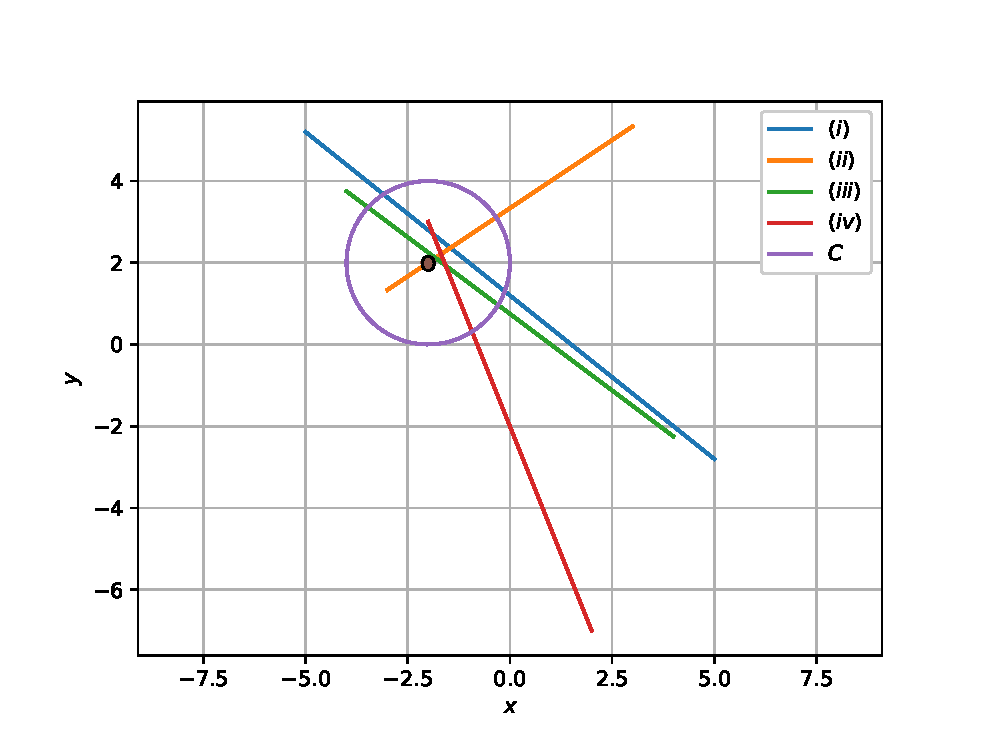
\includegraphics[width=0.6\columnwidth]{./figs/circle_diameter.eps}
%\caption{Circle $C$ and all lines (i)-(iv). (ii) is a diameter.}
%\label{fig:circle_diameter}
%\end{figure}
\end{frame}
%\begin{frame}
%\frametitle{Introduction}
%\framesubtitle{Literature}
%%\begin{figure}[t!]
%%    \centering
%%    \begin{subfigure}[t]{0.4\columnwidth}
%%        \centering
%%        \includegraphics[width=\columnwidth]{point_source}
%%        \caption{Single point source}
%%\label{fig3:subfig1}        
%%    \end{subfigure}%
%%    ~ 
%%    \begin{subfigure}[t]{0.4\columnwidth}
%%        \centering
%%        \includegraphics[width=\columnwidth]{pointNoPowerDist_new}
%%        \caption{SNR profile}
%%\label{fig3:subfig2}
%%    \end{subfigure}
%%  %  \caption{Average SNR for a BPP. $N=16$}
%%    \label{fig3}
%%  \end{figure}
%
%\end{frame}
%  
%
%
%%

\end{document}
